\documentclass{article}

\usepackage[T1]{fontenc}

\usepackage[spanish]{babel}


% Set page size and margins
% Replace `letterpaper' with `a4paper' for UK/EU standard size
\usepackage[letterpaper,top=2cm,bottom=2cm,left=3cm,right=3cm,marginparwidth=1.75cm]{geometry}

% Useful packages
\usepackage{amsmath}
\usepackage{graphicx}
\usepackage[colorlinks=true, allcolors=blue]{hyperref}
\usepackage{titling}

% Useful for augmented matrix representation
\makeatletter
\renewcommand*\env@matrix[1][*\c@MaxMatrixCols c]{%
  \hskip -\arraycolsep
  \let\@ifnextchar\new@ifnextchar
  \array{#1}}
\makeatother

\usepackage{listings}
\usepackage{color}

\definecolor{dkgreen}{rgb}{0,0.6,0}
\definecolor{gray}{rgb}{0.5,0.5,0.5}
\definecolor{mauve}{rgb}{0.58,0,0.82}

\lstset{frame=tb,
  language=Matlab,
  aboveskip=3mm,
  belowskip=3mm,
  showstringspaces=false,
  columns=flexible,
  basicstyle={\small\ttfamily},
  numbers=none,
  numberstyle=\tiny\color{gray},
  keywordstyle=\color{blue},
  commentstyle=\color{dkgreen},
  stringstyle=\color{mauve},
  breaklines=true,
  breakatwhitespace=true,
  tabsize=3
}

\setcounter{section}{0}

\title{
\includegraphics[scale=0.5]{logo.jpg}\\ \textbf{Laboratorio 2} 
\\ \large Resolución de Sistemas Lineales            
\\ \large Métodos de Computación Científica}

\author{Manuel Lagos}

\begin{document}
\maketitle

\section{Ejercicio 1}
$1.11$ Utilizar la eliminación de Gauss generando la descomposición $A=LU$ para resolver el sistema $Ax=b$, donde: \\
\[
A=\begin{bmatrix}
2 & 4 & -2 \\
4 & 9 & -3 \\
-2 & -1 & 7 \\
\end{bmatrix} \hspace{1cm}
b=\begin{bmatrix}
2 \\
8 \\
10 \\
\end{bmatrix}
\]\\

0. El sistema tiene solución y es única puesto que:

\[\begin{pmatrix}
2 & 4 & -2 \\
4 & 9 & -3 \\
-2 & -1 & 7 \\
\end{pmatrix} = 4 \neq 0\]\\

1. La matriz A se puede transformar en una matriz triangular superior U con la siguiente transformación T:

\[
\begin{bmatrix}
1 & 0 & 0 \\
0 & 1 & 0 \\
0 & 7 & 1 \\
\end{bmatrix}
\cdot
\begin{bmatrix}
1 & 0 & 0 \\
-\dfrac{1}{2} & 1 & 0 \\
\dfrac{1}{2} & 0 & 1 \\
\end{bmatrix}
\cdot
\begin{bmatrix}
0 & 1 & 0 \\
1 & 0 & 0 \\
0 & 0 & 1 \\
\end{bmatrix}
\cdot
\begin{bmatrix}
2 & 4 & -2 \\
4 & 9 & -3 \\
-2 & -1 & 7 \\
\end{bmatrix}
=
\begin{bmatrix}
4 & 9 & -3 \\
0 & -\dfrac{1}{2} & -\dfrac{1}{2} \\
0 & 0 & 2 \\
\end{bmatrix} = U
\]
\[
T =
\begin{bmatrix}
1 & 0 & 0 \\
0 & 1 & 0 \\
0 & 7 & 1 \\
\end{bmatrix}
\cdot
\begin{bmatrix}
1 & 0 & 0 \\
-\dfrac{1}{2} & 1 & 0 \\
\dfrac{1}{2} & 0 & 1 \\
\end{bmatrix} 
\cdot
\begin{bmatrix}
0 & 1 & 0 \\
1 & 0 & 0 \\
0 & 0 & 1 \\
\end{bmatrix}
\]
\[
T \cdot A = U
\]
2. El sistema puede ser vuelto a expresar como: \\
\[
    A \cdot x = b  
\]
\[
    T \cdot A \cdot x = T \cdot b  
\]
\[
    U \cdot x = T \cdot b  
\]
\[
    T \cdot b =
    \begin{bmatrix}
    8 \\
    -2 \\
    0 \\
    \end{bmatrix}
\]
\[ 
\begin{bmatrix}
4 & 9 & -3 \\
0 & -\dfrac{1}{2} & -\dfrac{1}{2} \\
0 & 0 & 2 \\
\end{bmatrix}
\cdot x = 
\begin{bmatrix}
8 \\
-2 \\
0 \\
\end{bmatrix}
\]\\
3. La matriz del sistema apliada es:
\[ 
\begin{bmatrix}[ccc|c]
  4 & 9 & -3 & 8\\
  0 & -\dfrac{1}{2} & -\dfrac{1}{2} & -2\\
  0 & 0 & 2 & 0
\end{bmatrix}\\
\]\\

4. Por sustitución hacia atrás:

\[
2 \cdot x3 = 0 \\
\]
\[
x3=0
\]

\[
-\dfrac{1}{2} \cdot x2 + -\dfrac{1}{2} \cdot x3 = -2 \\
\]
\[
-\dfrac{1}{2} \cdot x2 + -\dfrac{1}{2} \cdot 0 = -2 \\
\]
\[
x2 = -2 \cdot -2
\]
\[
x2 = 4  
\]

\[
4 \cdot x1 + 9 \cdot x2 - 3 \cdot x3 = 8 \\
\]
\[
4 \cdot x1 + 9 \cdot 4 + - 3 \cdot 0 = 8 \\
\]
\[
4 \cdot x1 + 36 = 8 \\
\]
\[
4 \cdot x1 = -28 \\
\]
\[
x1 = -28 \cdot \dfrac{1}{4}
\]
\[
x1 = -7
\]

Luego la solución del sistema es:
\[
    x =
    \begin{bmatrix}
    -7 \\
    4 \\
    0 \\
    \end{bmatrix}
\]\\

$1.12$ Utilizar la factorización $LU$ de $A$ computada en el inciso anterior para resolver el sistema $A \cdot y = c$.
\[
c=\begin{bmatrix}
4 \\
8 \\
-6 \\
\end{bmatrix}
\]\\
0. Como se demostró en el incisio anterior, el sistema tiene solución y es única. \\\\
1. Utilizando los resultados del inciso anterior se tiene que:\\
\[
U = T \cdot A
\]
Luego A se puede factorizar como:
\[
T^{-1} \cdot U = A
\]
\\
\[
A \cdot y = c
\]
\[
T^{-1} \cdot U \cdot y = c 
\]
\[
U \cdot y = T \cdot c
\]

\[
    T \cdot c = 
    \begin{bmatrix}
    8 \\
    0 \\
    -2 \\
    \end{bmatrix}
\] 
\[
\begin{bmatrix}
4 & 9 & -3 \\
0 & -\dfrac{1}{2} & -\dfrac{1}{2} \\
0 & 0 & 2 \\
\end{bmatrix}
\cdot y =
\begin{bmatrix}
8 \\
0 \\
-2 \\
\end{bmatrix}
\]\\

2. La matriz ampliada del nuevo sistema es:

\[ 
\begin{bmatrix}[ccc|c]
  4 & 9 & -3 & 8\\
  0 & -\dfrac{1}{2} & -\dfrac{1}{2} & 0\\
  0 & 0 & 2 & -2
\end{bmatrix}\\
\]\\

3. Por sustitución hacia atrás:
\[
2 \cdot y3 = -2 \\
\]
\[
y3=-1
\]

\[
-\dfrac{1}{2} \cdot y2 + -\dfrac{1}{2} \cdot y3 = 0 \\
\]
\[
-\dfrac{1}{2} \cdot y2 + -\dfrac{1}{2} \cdot -1 = 0 \\
\]
\[
y2 = -\dfrac{1}{2} \cdot -2
\]
\[
y2 = 1
\]

\[
4 \cdot y1 + 9 \cdot y2 - 3 \cdot y3 = 8 \\
\]
\[
4 \cdot y1 + 9 \cdot 1 + - 3 \cdot -1 = 8 \\
\]
\[
4 \cdot y1 + 12 = 8 \\
\]
\[
4 \cdot y1 = -4 \\
\]
\[
y1 = -4 \cdot \dfrac{1}{4}
\]
\[
y1 = -1
\]

La solución del sistema es:
\[
    y =
    \begin{bmatrix}
    -1 \\
    1 \\
    -1 \\
    \end{bmatrix}
\]\\

\section{Ejercicio 2}
Dada la siguiente matriz:

\begin{figure}[H]
    \centering
    
\includegraphics[width=1\linewidth]{Screenshot_20231008_190326.png}
    \label{fig:enter-label}
\end{figure}

2.1 ¿Qué sucede cuando se emplea Eliminación de Gauss con pivoteo parcial para
resolución de sistemas Ax = b? ¿Crecen los elementos de la matriz transformada? ¿Qué
sucede si se usa pivoteo completo en vez del parcial?\\
2.2 Emplee rutinas del MATLAB para resolver sistemas lineales de esta forma con el
método de eliminación de Gauss con pivoteo parcial, usando del lado derecho vectores
b tales que la solución sea conocida. ¿Cómo se comportan el error, el residuo y el
número de condición a medida que el sistema se agranda?\\
2.3 Con respecto al pivoteo, qué conclusiones se pueden sacar de los experimentos
realizados en 2.2? \\\\
\textbf{Aclaración}\\
Para la resolución del ejercicio se implementaron tres programas en Octave: uno que realiza pivoteo parcial por filas, otro por columnas, y otro completo. A continuación se exponen los resultados obtenidos para cada inciso y al final el código de los tres programas utilizados.\\

2.1 
El pivoteo parcial, ya sea por filas o por columnas, se emplea para evitar la aparición de divisiones por cero, o números cercanos a cero, y para reducir el error numérico en el proceso de eliminación. El pivoteo completo, por otro lado, es una variante más avanzada del método que busca minimizar aún más los errores numéricos, considerando todos los elementos de la matriz.\\ 

En el caso de la matriz A dada, el pivoteo parcial por filas escala los elementos de la matriz transformada considerablemente. En cambio en el pivoteo parcial por columnas y el pivoteo completo, equivalentes en este caso particular, el factor de crecimiento es menor.\\

El factor de crecimiento de una matriz A de n x n con la eliminación de Gauss se define como 
\[
G_n(A) = \dfrac{\max_{i, j, k}{|a_{ij}^{(k)}|}}{\max_{i, j}{|a_{ij}|}}
\]\\
Esta variable es una medida de la estabilidad numérica de la solución al sistema $A \cdot x = b$.\\

\textit{[Kincaid] (2002) Numerical Analysis Mathematics of Scientific Computing - Chapter Four \\}

Resultado:

\begin{lstlisting}
    PivoteoParcialFilas =
    1    0    0    0    1
    0    1    0    0    2
    0    0    1    0    4
    0    0    0    1    8
    0    0    0    0   16

    ㅤ
    ㅤ
    ㅤ
    
    PivoteoParcialColumnas =
    1   1   0   0   0
    0   2   1   0   0
    0   0  -2   1   0
    0   0   0  -2   1
    0   0   0   0  -2


    PivoteoCompleto
    1   1   0   0   0
    0   2   1   0   0
    0   0  -2   1   0
    0   0   0  -2   1
    0   0   0   0  -2

\end{lstlisting}

2.2 
Se realizó una bateria de experimentos para cada método, monitoreando el error y el residuo obtenido, así también como el tiempo de ejecución. Los vectores solución fueron generados aleatoriamente, pero la experiencia puede repetirse ejecutando el código presentado.

\begin{lstlisting}
% probando el método de eliminación de gauss para sistemas lineales con pivoteo parcial
exp 1. la norma del error es 4.742875E-16 y la norma del residuo 7.364386E-16
exp 2. la norma del error es 3.597534E-16 y la norma del residuo 5.768888E-16
exp 3. la norma del error es 1.271920E-16 y la norma del residuo 1.922963E-16
exp 4. la norma del error es 2.860979E-16 y la norma del residuo 6.753223E-16
exp 5. la norma del error es 2.371437E-16 y la norma del residuo 3.330669E-16
exp 6. la norma del error es 2.963485E-16 y la norma del residuo 4.299875E-16
exp 7. la norma del error es 1.927964E-16 y la norma del residuo 3.330669E-16
exp 8. la norma del error es 1.837170E-16 y la norma del residuo 3.845925E-16
exp 9. la norma del error es 6.973502E-17 y la norma del residuo 1.110223E-16
exp 10. la norma del error es 2.371437E-16 y la norma del residuo 3.682193E-16
exp 11. la norma del error es 2.237726E-16 y la norma del residuo 3.330669E-16
exp 12. la norma del error es 3.188873E-16 y la norma del residuo 5.768888E-16
exp 13. la norma del error es 1.359740E-16 y la norma del residuo 1.922963E-16
exp 14. la norma del error es 6.359601E-17 y la norma del residuo 0.000000E+00
exp 15. la norma del error es 4.785322E-16 y la norma del residuo 6.661338E-16
exp 16. la norma del error es 6.158048E-16 y la norma del residuo 8.741905E-16
exp 17. la norma del error es 3.608225E-16 y la norma del residuo 4.154074E-16
exp 18. la norma del error es 1.012698E-16 y la norma del residuo 1.570092E-16
exp 19. la norma del error es 1.241267E-16 y la norma del residuo 3.140185E-16
exp 20. la norma del error es 8.821952E-16 y la norma del residuo 1.304217E-15
Elapsed time is 0.0176399 seconds.

% probando el método de eliminación gauss para sistemas lineales con pivoteo completo
exp 1. la norma del error es 1.688306E-16 y la norma del residuo 2.482534E-16
exp 2. la norma del error es 1.177569E-16 y la norma del residuo 1.570092E-16
exp 3. la norma del error es 6.938894E-17 y la norma del residuo 1.110223E-16
exp 4. la norma del error es 9.614813E-17 y la norma del residuo 2.719480E-16
exp 5. la norma del error es 9.309503E-17 y la norma del residuo 1.570092E-16
exp 6. la norma del error es 2.775558E-17 y la norma del residuo 1.665335E-16
exp 7. la norma del error es 6.206335E-17 y la norma del residuo 1.241267E-16
exp 8. la norma del error es 4.163336E-17 y la norma del residuo 5.551115E-17
exp 9. la norma del error es 0.000000E+00 y la norma del residuo 1.665335E-16
exp 10. la norma del error es 8.326673E-17 y la norma del residuo 2.220446E-16
exp 11. la norma del error es 1.110223E-16 y la norma del residuo 1.570092E-16
exp 12. la norma del error es 1.103699E-16 y la norma del residuo 1.755417E-16
exp 13. la norma del error es 1.144392E-16 y la norma del residuo 1.570092E-16
exp 14. la norma del error es 2.775558E-17 y la norma del residuo 0.000000E+00
exp 15. la norma del error es 1.387779E-17 y la norma del residuo 1.271920E-16
exp 16. la norma del error es 6.206335E-17 y la norma del residuo 1.570092E-16
exp 17. la norma del error es 2.775558E-17 y la norma del residuo 0.000000E+00
exp 18. la norma del error es 8.326673E-17 y la norma del residuo 1.144392E-16
exp 19. la norma del error es 4.163336E-17 y la norma del residuo 0.000000E+00
exp 20. la norma del error es 1.209837E-16 y la norma del residuo 1.570092E-1
Elapsed time is 0.077153 seconds.

>> cond(A)
ans = 10.763

% el número de condición de la matriz transformada no es demasiado alto
\end{lstlisting}

2.3
De los experimentos realizados podemos concluir que el pivoteo completo, si bien obtiene mejores resultados que el pivoteo parcial, tiene un alto costo computacional, con orden asintótico de $(p - r + 1)^2$ comparaciones frente a $(p - r + 1)$. Dependerá del caso puntual de aplicación cuál técnica utilizar, según se quiera alcanzar mayor precisión o mayor rendimiento. \\

A continuación el código de los tres programas:\\

P1: Pivoteo parcial por filas.
\begin{lstlisting}
clc; % limpiar la pantalla

function [A, b] = gaussConPivoteoParcialFilas(A, b)
  [n, m] = size(A);

  if n != m || n != size(b)
    A = zeros(n,m);
    printf("ERROR: la matriz debe ser cuadrada y coincidir con la dimensión de b\n");
    return;
  end

  for i=1:n
    % pivotear parcialmente por filas
    max = abs(A(i, i));
    fila = i;
    P = eye(n, n);

    for k=i:n
      if abs(A(k, i)) > max
        max = abs(A(k, i));
        fila = k;
      end
    end

    % permutar filas
    aux = A(i, 1:n);
    A(i, 1:n) = A(fila, 1:n);
    A(fila, 1:n) = aux;
    aux = b(i);
    b(i) = b(fila);
    b(fila) = aux;

    % triangular
    for k=i+1:n
      escalar = (A(k, i)/A(i, i));
      A(k, 1:n) = A(k, 1:n) -  (A(i, 1:n) .* escalar);
      b(k) = b(k) - (b(i) * escalar);
    end
  end
end

function x = sustHaciaAtras(A, b)
  [n, m] = size(A);
  x = zeros(1, n); % vector de resultados

  if n != m || n != size(b)
    A = zeros(n,m);
    printf("ERROR: la matriz debe ser cuadrada y coincidir con la dimensión de b\n");
    return;
  end

  for i= [n:-1:1] % recorrer la matriz de abajo hacia arriba
    aux = 0; % suma de cada x_j de la fila por cada coeficiente
             % en base a resultados anteriores

    for j=i+1:n   % recorrer la fila hacia derecha
      if j != i
        aux += A(i, j) * x(j); % agregar x_j * a(i, j)
      end
    end

    x(i) = (b(i)- aux)/A(i, i); % calcular el nuevo x_i
  end
  x = x'; % devolver como vector columna
end

function [] = testear(n)
  display("probando el método de eliminación de gauss para sistemas lineales con pivoteo parcial");

  tic % controlar tiempo de ejecución

  A = [ 1, 0, 0, 0, 1;
     -1, 1, 0, 0, 1;
     -1,-1, 1, 0, 1;
     -1,-1,-1, 1, 1;
     -1,-1,-1,-1, 1 ];

  for i=1:n
     b = rand(1,5)'; % generar un vector aleatorio para los térs. ind.
     x = inv(A) * b; % obtener la solución del sistema

     [A2, b2] = gaussConPivoteoParcialFilas(A, b); % obtener el pivoteo
     x2 = sustHaciaAtras(A2, b2); % realizar la sustitución

     error = norm(x - x2); % computar el error
     residuo = norm((A * x2) - b); % computar el residuo

     printf("exp %d. la norma del error es %E y la norma del residuo %E\n", i, error, residuo);
  end

  toc % fin tiempo de ejecución
end

testear(20);
\end{lstlisting}
\\

P2: Pivoteo Parcial por columnas.
\begin{lstlisting}
clc; % limpiar la pantalla

function [A, b, VP] = gaussConPivoteoParcialColumnas(A, b)
  [n, m] = size(A);
  VP = [1:n]; % vector de permutaciones de cols

  if n != m || n != size(b)
    A = zeros(n,m);
    printf("ERROR: la matriz debe ser cuadrada y coincidir con la dimensión de b\n");
    return;
  end

  for i=1:n
    % pivotear por columnas
    max = abs(A(i, i));
    col = i;
    P = eye(n, n);

    for m=i:n
        if abs(A(i, m)) > max
          max = abs(A(i, m));
          col = m;
        end
    end

    % permutar columnas
    aux = A(1:n, i);
    A(1:n, i) = A(1:n, col);
    A(1:n, col) = aux;

    % guardar vector de permutación para las incógnitas
    aux = VP(i);
    VP(i) = VP(col);
    VP(col) = aux;

    % triangular
    for k=i+1:n
      escalar = (A(k, i)/A(i, i));
      A(k, 1:n) = A(k, 1:n) -  (A(i, 1:n) .* escalar);
      b(k) = b(k) - (b(i) * escalar);
    end
  end

  VP = VP';
end

function x = sustHaciaAtras(A, b)
  [n, m] = size(A);
  x = zeros(1, n); % vector de resultados

  if n != m || n != size(b)
    A = zeros(n,m);
    printf("ERROR: la matriz debe ser cuadrada y coincidir con la dimensión de b\n");
    return;
  end

  for i= [n:-1:1] % recorrer la matriz de abajo hacia arriba
    aux = 0; % suma de cada x_j de la fila por cada coeficiente
             % en base a resultados anteriores

    for j=i+1:n   % recorrer la fila hacia derecha
      if j != i
        aux += A(i, j) * x(j); % agregar x_j * a(i, j)
      end
    end

    x(i) = (b(i)- aux)/A(i, i); % calcular el nuevo x_i
  end
  x = x'; % devolver como vector columna
end

% permutar un vector según un vector de permutación VP
function xp = permutarVector(x, VP)
  [n, m] = size(x);

  if size(x) != size(VP)
    printf("ERROR: las dimensiones del vector y el vec. de permutación no coinciden\n");
    return;
  end

  xp = zeros(1, n); % vector permutado

  for i=1:n
    xp(VP(i)) = x(i); % reescribir el vector x según el vector de permutación
  end

  xp = xp'; % devolver como vector columna
end
\end{lstlisting}

P3: Pivoteo Completo.
\begin{lstlisting}
clc; % limpiar la pantalla

function [A, b, VP] = gaussConPivoteoCompleto(A, b)
  [n, m] = size(A);
  VP = [1:n]; % vector de permutaciones de cols

  if n != m || n != size(b)
    A = zeros(n,m);
    printf("ERROR: la matriz debe ser cuadrada y coincidir con la dimensión de b\n");
    return;
  end

  for i=1:n
    % pivotear completo
    max = abs(A(i, i));
    pos = [i, i];
    P = eye(n, n);

    for k=i:n
      for m=i:n
        if abs(A(k, m)) > max
          max = abs(A(k, m));
          pos = [k, m];
        end
      end
    end

    % permutar filas
    aux = A(i, 1:n);
    A(i, 1:n) = A(pos(1), 1:n);
    A(pos(1), 1:n) = aux;
    aux = b(i);
    b(i) = b(pos(1));
    b(pos(1)) = aux;

    % permutar columnas
    aux = A(1:n, i);
    A(1:n, i) = A(1:n, pos(2));
    A(1:n, pos(2)) = aux;

    % guardar vector de permutación para las incógnitas
    aux = VP(i);
    VP(i) = VP(pos(2));
    VP(pos(2)) = aux;

    % triangular
    for k=i+1:n
      escalar = (A(k, i)/A(i, i));
      A(k, 1:n) = A(k, 1:n) -  (A(i, 1:n) .* escalar);
      b(k) = b(k) - (b(i) * escalar);
    end
  end
end

function x = sustHaciaAtras(A, b)
  [n, m] = size(A);
  x = zeros(1, n); % vector de resultados

  if n != m || n != size(b)
    A = zeros(n,m);
    printf("ERROR: la matriz debe ser cuadrada y coincidir con la dimensión de b\n");
    return;
  end

  for i= [n:-1:1] % recorrer la matriz de abajo hacia arriba
    aux = 0; % suma de cada x_j de la fila por cada coeficiente
             % en base a resultados anteriores

    for j=i+1:n   % recorrer la fila hacia derecha
      if j != i
        aux += A(i, j) * x(j); % agregar x_j * a(i, j)
      end
    end

    x(i) = (b(i)- aux)/A(i, i); % calcular el nuevo x_i
  end
  x = x'; % devolver como vector columna
end

% permutar un vector según un vector de permutacion VP
function xp = permutarVector(x, VP)
  [n, m] = size(x);

  if size(x) != size(VP)
    printf("ERROR: las dimensiones del vector y el vec. de permutación no coinciden\n");
    return;
  end

  xp = zeros(1, n); % vector permutado

  for i=1:n
    xp(VP(i)) = x(i); % reescribir el vector x según el vector de permutación
  end

  xp = xp'; % devolver como vector columna
end

function [] = testear(n)
  display("probando el método de eliminación de gauss para sistemas lineales con pivoteo completo");

  tic % controlar tiempo de ejecución

  A = [ 1, 0, 0, 0, 1;
     -1, 1, 0, 0, 1;
     -1,-1, 1, 0, 1;
     -1,-1,-1, 1, 1;
     -1,-1,-1,-1, 1 ];

  for i=1:n
     b = rand(1,5)'; % generar un vector aleatorio para los térs. ind.
     x = inv(A) * b; % obtener la solución del sistema

     [A2, b2, PV] = gaussConPivoteoCompleto(A, b); % obtener el pivoteo
     x2 = sustHaciaAtras(A2, b2); % realizar la sustitución
     x2 = permutarVector(x2, PV');
     error = norm(x - x2); % computar el error
     residuo = norm((A * x2) - b); % computar el residuo

     printf("exp %d. la norma del error es %E y la norma del residuo %E\n", i, error, residuo);
  end

  toc % fin tiempo de ejecución
end

testear(20);
\end{lstlisting}
\\


\section{Ejercicio 3}
\[
A=\begin{bmatrix}
5 & 3 & -2 \\
3 & 2 & -2 \\
-2 & -2 & 5 \\
\end{bmatrix} 
\hspace{1cm}
B=\begin{bmatrix}
2 & 3 & -1 \\
3 & 4 & -2 \\
-1 & -2 & 1 \\
\end{bmatrix}
\]\\

3.1 Cuál de estas dos matrices es definida positiva? Use el cálculo de determinantes para encontrar su respuesta a esta pregunta.\\\\
El criterio de Sylvester dice que si todas las menores principales de $A \in\Re^{n \cdot n}$ son positivas entonces A es definida positiva, esto es: $x^{T} \cdot A \cdot x > 0 ,\forall x \in \Re^n$.
\[
\begin{pmatrix}
5
\end{pmatrix} 
= 5 > 0
\]
\[
\begin{pmatrix}
5 & 3 \\
3 & 2 \\
\end{pmatrix} 
= 5 \cdot 2 - 3 \cdot 3 = 1 > 0
\]
\[
\begin{pmatrix}
5 & 3 & -2 \\
3 & 2 & -2 \\
-2 & -2 & 5 \\
\end{pmatrix} =
\]
\[
(5 \cdot 2 \cdot 5 + 3 \cdot -2 \cdot -2 + 3 \cdot -2 \cdot -2) - 
(-2 \cdot 2 \cdot -2 + 3 \cdot 3 \cdot 5 + -2 \cdot -2 \cdot 5) =
\]
\[
74 - 73 = 1 > 0
\]

Luego A es definida positiva.\\

\[
\begin{pmatrix}
2
\end{pmatrix} 
= 2 > 0
\]
\[
\begin{pmatrix}
2 & 3 \\
3 & 4 \\
\end{pmatrix} 
= 2 \cdot 4 - 3 \cdot 3 = -1 < 0
\]

\[
\begin{pmatrix}
2 & 3 & -1 \\
3 & 4 & -2 \\
-1 & -2 & 1 \\
\end{pmatrix} =
\]

\[
(2 \cdot 4 \cdot 1 + 3 \cdot -2 \cdot -1 + 3 \cdot -2 \cdot -1) - 
(-1 \cdot 4 \cdot -1 + 2 \cdot -2 \cdot -2 + 3 \cdot 3 \cdot 1) =
\]
\[
20 - 21 = -1 < 0
\]

Luego B no es definida positiva.\\

3.2 Muestre que $x̅ = \begin{bmatrix}1 & -1 & 1\end{bmatrix}^{T}$ es la solución de estos sistemas:
$A \cdot x = \begin{bmatrix}0 & -1 & 5\end{bmatrix}^{T}$ y $B \cdot x = \begin{bmatrix}-2 & -3 & 2\end{bmatrix}^{T}.

\[
A \cdot \begin{bmatrix}1 & -1 & 1\end{bmatrix}^{T} = 
\begin{bmatrix}x_1 & x_2 & x_3 \end{bmatrix}^{T}
\]

\[
\begin{bmatrix}
5 & 3 & -2 \\
3 & 2 & -2 \\
-2 & -2 & 5 \\
\end{bmatrix} 
\cdot
\begin{bmatrix}
1 \\ -1 \\ 1
\end{bmatrix} 
=
\begin{bmatrix}
x_1 \\ x_2 \\ x_3
\end{bmatrix} 
\]

\[
x_1 = 5 \cdot 1 + 3 \cdot -1 + -2 \cdot 1 = 5 - 3 - 2 = 0 
\]

\[
x_2 = 3 \cdot 1 + 2 \cdot -1 + -2 \cdot 1 = 3 - 2 - 2 = -1 
\]

\[
x_3 = -2 \cdot 1 + -2 \cdot -1 + 5 \cdot 1 = -2 + 2 + 5 = 5 
\]

\[
x =
\begin{bmatrix}
    0 \\ -1 \\ 5
\end{bmatrix} 
\]

\[
B \cdot \begin{bmatrix}1 & -1 & 1\end{bmatrix}^{T} = 
\begin{bmatrix}x'_1 & x'_2 & x'_3 \end{bmatrix}^{T}
\]

\[
\begin{bmatrix}
2 & 3 & -1 \\
3 & 4 & -2 \\
-1 & -2 & 1 \\
\end{bmatrix} 
\cdot
\begin{bmatrix}
1 \\ -1 \\ 1
\end{bmatrix} 
=
\begin{bmatrix}
x'_1 \\ x'_2 \\ x'_3
\end{bmatrix} 
\]

\[
x'_1 = 2 \cdot 1 + 3 \cdot -1 + -1 \cdot 1 = 2 -3 - 1 = -2 
\]

\[
x'_2 = 3 \cdot 1 + 4 \cdot -1 + -2 \cdot 1 = 3 - 4 - 2 = -3 
\]

\[
x'_3 = -1 \cdot 1 + -2 \cdot -1 + 1 \cdot 1 = -1 + 2 + 1 = 2 
\]

\[
x' =
\begin{bmatrix}
    -2 \\ -3 \\ 2
\end{bmatrix} 
\]\\
 
3.3 Resuelva estos dos sistemas usando el método de Choleski donde corresponda. Caso
contrario, realice dos iteraciones por el método de Gauss Seidel comenzando con
$x_0 = [0 \hspace{0.1cm} 0 \hspace{0.1cm} 0]^{T}$ \\\\
Como tanto A como B tienen determinante distinto de 0, luego los sistemas tienen solución y es única.
Dado que la matriz A es simétrica, definida positiva y real, es posible resolver el sistema por el método de Cholesky. No es así con B.\\

1. Resolución del sistema $A \cdot x = b$ por el método de Cholesky:

\[
A \cdot x = b
\]
\[
L \cdot U \cdot x = b
\]
\[
U \cdot x = L^{-1} \cdot b = y
\]
\[
b = L \cdot y
\]

El método de Cholesky consdiera $U = L^T$ 

\[
L \cdot L^T = A
\]

\[
\begin{bmatrix}
l_{11} & 0 & 0 \\
l_{21} & l_{22} & 0 \\
l_{31} & l_{32} & l_{33} \\
\end{bmatrix} 
\cdot
\begin{bmatrix}
l_{11} & l_{21} & l_{31} \\
0 & l_{22} & l_{32} \\
0 & 0 & l_{33} \\
\end{bmatrix} 
=
\begin{bmatrix}
5 & 3 & -2 \\
3 & 2 & -2 \\
-2 & -2 & 5 
\end{bmatrix} 
\]

\[
5 = l_{11} \cdot l_{11} + 0 \cdot 0 + 0 \cdot 0 \implies l_{11} = \sqrt{5}
\]
\[
3 = l_{21} \cdot l_{11} + l_{22} \cdot 0 + 0 \cdot 0 
  = l_{21} \cdot \sqrt{5} 
\implies l_{21} = \dfrac{3}{\sqrt{5}}
\]

\[
2 = l_{21} \cdot l_{21} + l_{22} \cdot l_{22} + 0 \cdot 0 
  = \dfrac{9}{5} + l_{22} \cdot l_{22} 
\implies l_{22} = \sqrt{\dfrac{1}{5}}
\]

\[
-2 = l_{31} \cdot l_{11} + l_{32} \cdot 0 + l_{33} \cdot 0 
= l_{31} \cdot \sqrt{5} 
\implies l_{31} = \dfrac{-2}{\sqrt{5}}
\]

\[
-2 = l_{31} \cdot l_{21} + l_{32} \cdot l_{22} + l_{33} \cdot 0 
= \dfrac{-2}{\sqrt{5}} \cdot \dfrac{3}{\sqrt{5}} + l_{32} \cdot \sqrt{\dfrac{1}{5}} +
\implies l_{32} = \dfrac{\dfrac{-4}{5}}{\sqrt{\dfrac{1}{5}}}
\]

\[
5 = l_{31} \cdot l_{31} + l_{32} \cdot l_{32} + l_{33} \cdot l_{33}
= \dfrac{-4}{5} + \dfrac{\dfrac{16}{25}}{\dfrac{1}{5}} + l_{33} \cdot l_{33}
= \dfrac{4}{5} + \dfrac{16}{5} + l_{33} \cdot l_{33}
= 4 + l_{33} \cdot l_{33}
\implies l_{33} = 1
\]

\[
\begin{bmatrix}
\sqrt{5} & 0 & 0 \\
\dfrac{3}{\sqrt{5}} & \sqrt{\dfrac{1}{5}} & 0 \\
\dfrac{-2}{\sqrt{5}} & \dfrac{-4}{\sqrt(5)} & 1 \\
\end{bmatrix} 
\cdot
\begin{bmatrix}
\sqrt{5} & \dfrac{3}{\sqrt{5}} & \dfrac{-2}{\sqrt{5}} \\
0 & \sqrt{\dfrac{1}{5}} & \dfrac{-4}{\sqrt(5)} \\
0 & 0 & 1 \\
\end{bmatrix} 
=
\begin{bmatrix}
5 & 3 & -2 \\
3 & 2 & -2 \\
-2 & -2 & 5 
\end{bmatrix} 
\]\\

Resolución del sistema
\[
L \cdot y = b
\]

La matriz ampliada es:

\[ 
\begin{bmatrix}[ccc|c]
  \sqrt{5} & 0 & 0 & 0\\ 
\dfrac{3}{\sqrt{5}} & \sqrt{\dfrac{1}{5}} & 0 & -1\\
\dfrac{-2}{\sqrt{5}} & \dfrac{-4}{\sqrt(5)} & 1 & 5 \\
\end{bmatrix}\\
\]\\

Por sustitución hacia adelante:
\[
\sqrt{5} \cdot y_1 = 0 \implies y_1 = 0
\]

\[
\sqrt{\dfrac{1}{5}} \cdot y_2 = -1 \implies y_2 = \dfrac{-1}{\sqrt{\dfrac{1}{5}}} = -\sqrt{5}
\]

\[
\dfrac{-4}{\sqrt{5}} \cdot -\sqrt{5}
+ 1 \cdot y_3 = 
4 + 1 \cdot y_3 = 
5 \implies y_3 = 1
\]

La solución del sistema es:
\[
    y =
    \begin{bmatrix}
    0 \\
    -\sqrt{5} \\
    1 \\
    \end{bmatrix}
\]\\

\[
U \cdot x = y
\]
\[
L^T \cdot x = y
\]
\[
\begin{bmatrix}
\sqrt{5} & \dfrac{3}{\sqrt{5}} & \dfrac{-2}{\sqrt{5}} \\
0 & \sqrt{\dfrac{1}{5}} & \dfrac{-4}{\sqrt(5)} \\
0 & 0 & 1 \\
\end{bmatrix} 
\cdot x = 
\begin{bmatrix}
    0 \\
    -\sqrt{5} \\
    1 \\
    \end{bmatrix}
\]\\

La matriz ampliada es:

\[ 
\begin{bmatrix}[ccc|c]
\sqrt{5} & \dfrac{3}{\sqrt{5}} & \dfrac{-2} {\sqrt{5}} & 0 \\
0 & \sqrt{\dfrac{1}{5}} & \dfrac{-4}{\sqrt(5)} &  -\sqrt{5}\\
0 & 0 & 1 & 1 \\
\end{bmatrix}\\
\]\\

Resolución del sistema por sustitución hacia atrás.

\[
x_3 \cdot 1 = 1 \implies x_3 = 1 
\]\\

\[
x_2 \cdot \sqrt{\dfrac{1}{5}} + x_3 \cdot \dfrac{-4}{\sqrt{5}} =
x_2 \cdot \sqrt{\dfrac{1}{5}} + \dfrac{-4}{\sqrt{5}} = -\sqrt{5}
\]
\[
x_2 \cdot \dfrac{1}{\sqrt{5}} + \dfrac{-4}{\sqrt{5}} = -\sqrt{5}
\implies x_2 = -1
\]\\

\[
x_1 \cdot \sqrt{5} + \dfrac{3}{\sqrt{5}} \cdot -1 + \dfrac{-2}{\sqrt{5}} \cdot 1 = 0
\]
\[
x_1 \cdot \sqrt{5} = \dfrac{5}{\sqrt{5}} \implies x_1 = 1
\]\\

Efectivamente la solución del sistema es:
\[
    x =
    \begin{bmatrix}
    1 \\
    -1 \\
    1 \\
    \end{bmatrix}
\]\\
\textbf{Aclaración}\\
2. Resolución del sistema $B \cdot x = b$ por el método de Gauss Seidel. Si bien la consigna no lo pedía, se analizó la convergencia del método para la matriz B. Dado que el radio espectral de la matriz de iteración de Gauss Seidel para B es mayor a 1, el método no converge. De todas formas se realizaron las dos iteraciones.

\begin{lstlisting}
>> B = [2,3,-1;3,4,-2;-1,-2,1]
B =

   2   3  -1
   3   4  -2
  -1  -2   1

>> [L, D, U] = descomponerLDU(B);
>> Mitr = -1 * inv(L + D) * U;
>> abs(eig(Mitr))
ans =

        0
   1.2965
   0.5785

\end{lstlisting}
$1.2965 = \rho(Mitr) > 1$, luego el método de Gauss Seidel no converge\\

Deducción:

\[
B \cdot x = b
\]

\[
(L + D + U) \cdot x = b
\]

\[
(L + D) \cdot x = -U \cdot x + b
\] \\

\[
(L + D) \cdot x^{k+1} = -U \cdot x^k + b
\] \\

Resolviendo este sistema se obtiene la nueva solución $x^{k+1}$. A continuación se realizan dos iteraciones, tomando como $x^0$ inicial a $\begin{bmatrix}
    0 & 0 & 0
\end{bmatrix}^T$.

1. Primera iteración

\[
(L + D) \cdot x^{1} = -U \cdot x^0 + b
\] 

\[ 
\begin{bmatrix}
2 & 0 & 0 \\
3 & 4 & 0 \\
-1 & -2 & 1 
\end{bmatrix} \cdot x^{1} = 
\begin{bmatrix}
0 & -3 & 1 \\
0 & 0 & 2 \\
0 & 0 & 0 
\end{bmatrix}
\cdot
\begin{bmatrix}
    0 \\ 0 \\ 0
\end{bmatrix}
+
\begin{bmatrix}
    -2 \\ -3 \\ 2
\end{bmatrix}
\]

\[ 
\begin{bmatrix}
2 & 0 & 0 \\
3 & 4 & 0 \\
-1 & -2 & 1 
\end{bmatrix} \cdot x^{1} = 
\begin{bmatrix}
    -2 \\ -3 \\ 2
\end{bmatrix}
\]
\[ 
\begin{bmatrix}[ccc|c]
2 & 0 & 0 & -2 \\
3 & 4 & 0 & -3 \\
-1 & -2 & 1 & 2 
\end{bmatrix}\\
\]
Por sustitución hacia adelante:
\[
x_1^1 = -1
\]
\[
x_2^1 = 0
\]
\[
x_3^1 = 1
\]\\

2. Segunda iteración

\[
(L + D) \cdot x^{2} = -U \cdot x^1 + b
\] 

\[ 
\begin{bmatrix}
2 & 0 & 0 \\
3 & 4 & 0 \\
-1 & -2 & 1 
\end{bmatrix} \cdot x^{1} = 
\begin{bmatrix}
0 & -3 & 1 \\
0 & 0 & 2 \\
0 & 0 & 0 
\end{bmatrix}
\cdot
\begin{bmatrix}
    -1 \\ 0 \\ 1
\end{bmatrix}
+
\begin{bmatrix}
    -2 \\ -3 \\ 2
\end{bmatrix}
\]

\[ 
\begin{bmatrix}
2 & 0 & 0 \\
3 & 4 & 0 \\
-1 & -2 & 1 
\end{bmatrix} \cdot x^{1} = 
\begin{bmatrix}
    1 \\ 2 \\ 0
\end{bmatrix}
+
\begin{bmatrix}
    -2 \\ -3 \\ 2
\end{bmatrix}
\]
\[ 
\begin{bmatrix}[ccc|c]
2 & 0 & 0 & -1 \\
3 & 4 & 0 & -1 \\
-1 & -2 & 1 & 2 
\end{bmatrix}\\
\]
Por sustitución hacia adelante:
\[
x_1^2 = \dfrac{-1}{2}
\]
\[
x_2^2 = \dfrac{1}{8}
\]
\[
x_3^2 = \dfrac{7}{4}
\]\\

\[ x^2 = \begin{bmatrix}
    \dfrac{-1}{2} & \dfrac{1}{8} & \dfrac{7}{4}
\end{bmatrix}^T\]

Como puede apreciarse, el método no parece converger a la solución $\begin{bmatrix}
    1 & -1 & 1
\end{bmatrix}^T$.

\section{Ejercicio 4}
 Emplee los métodos de a) Jacobi y b) Gauss Seidel para resolver el sistema
lineal Ax = b para obtener una precisión de la solución en norma infinito menor o igual
que 10−5. Los elementos de A son:
\begin{figure}[H]
    \centering
    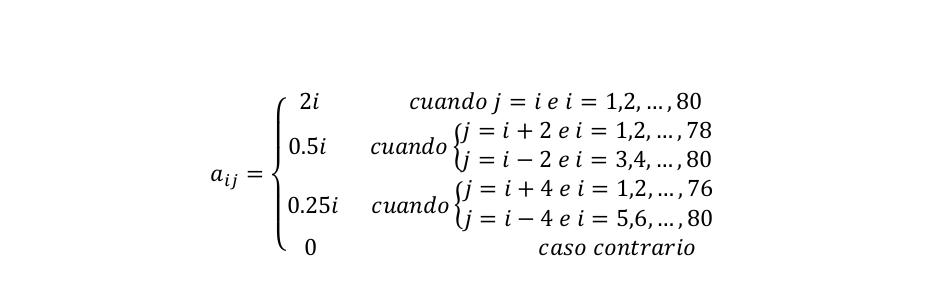
\includegraphics[width=1\linewidth]{Screenshot_20231008_160006.png}
    \label{fig:enter-label}
\end{figure}

Y los elementos de b son: bi = π para cada i = 1,2, ... ,80\\

\textbf{Aclaración}\\
El ejercicio se resolvió utilizando el software Octave. A continuación una dedución de cada método y la fórmula implementada en Octave. Luego el código y el resultado obtenido.\\

a) Jacobi

\[
A \cdot x = b
\]
\[
(L + D + U) \cdot x = b
\]
\[
(L + D + U) \cdot x = b
\]
\[
D \cdot x = b -(L + U) \cdot x
\]
\[
D \cdot x^{k+1} = -(L + U) \cdot x^k + b
\]

Resolviendo este sistema se encuentra la siguiente solución $x_{k+1}$.
Esto mismo puede implementare con la siguiente fórmula:

\[
x_i^{k+1} = \dfrac{1}{a_{11}} \cdot (b_i - \sum_{j=1, j \neq i}^n{a_{ij} \cdot x_j^k)
\]

Implementación en Octave

\begin{lstlisting}
clc; % limpiar la consola

% generar la matriz A y el vector b del enunciado
function [A, b] = generarMatriz(n)
  A = zeros(n);
  b = zeros(n, 1);

  for i = 1:n
    b(i) = pi;

    for j = 1:n
      el = 0;
      if j == i
        el = 2 * i;
      elseif j == i+2 && i<=78
        el = 0.5 * i;
      elseif j == i-2 && i>=3
        el = 0.5 * i;
      elseif j == i+4 && i<=76
        el = 0.25 * i;
      elseif j == i-4 && i>=5
        el = 0.25 * i;
      end
      A(i, j) = el;
    end
  end
end

% chequear si A es simétrica
function res = esSimetrica(A)
    res = A==A';
end

% chequear si A es definida positiva
function res = esDefPos(A)
    res = true;
    [n, m] = size(A);

    if n == m
        for i = 1:n
          if (det(A(1:i, 1:i)) <= 0)
           res = false;
           break
          end
        end
    end
end

% chequear si A es diagonal estricta por filas
function res = esDiagonalEstrictaFilas(A)
  [n, m] = size(A);
  res = true;

  for i = 1:n
  el = A(i, i);

    for j = 1:m
      if j != i && A(i, j)>=el
        res = false;
        break;
      end
    end
  end
end

% descomponer A en A = L + D + U
function [L, D, U] = descomponerLDU(A)
  D = A .* eye(size(A));
  L = A .* tril(ones(size(A)));
  U = A .* triu(ones(size(A)));
  L = L - D;
  U = U - D;
end

% comprobar si Jacobi converge
function res = convergeJacobi(A)
  res = false;

  [n, m] = size(A);
  if n != m
   return;
  end
                                         % el método de Jacobi converge si:
  if (esDiagonalEstrictaFilas(A))        % 1. A es diag. estric. por filas (cond. suf.)
    res = true;
  else
    [L, D, U] = descomponerLDU(A);
    Mitr = -1 * inv(D) * (L + U);        % 2. ||Mitr|| < 1 (cond. suf.)
    if (norm(Mitr) < 1)
        res = true;
    elseif (max(abs(eig(Mitr))) < 1)     % 3. ρ(Mitr) < 1 (cond. nec. y suf.)
        res = true;
    end
  end
end

% resolver Ax=b con el método de Jacobi a partir del x_anterior dado y hasta obtener cierto error.
function x_siguiente = jacobi(A, b, x_anterior, error)
   [n, m] = size(A);
   resto = 0;
   x_siguiente=x_anterior;

   if (n != m || n != size(b)(1) || size(b) != size(x_anterior)) % chequear las dimensiones de los argumentos
     fprintf("ERROR: La matriz debe ser cuadrada y coincidir con la dimensión de b y x_anterior\n");
   elseif convergeJacobi(A) % comprobar si el método de Jacobi converge
     resto = norm((A*x_siguiente)-b, Inf); % calcular el resto con norma infinito

     while (resto > error) % iterar hasta obtener el error deseado
       for i = 1:n
         aux = 0; %calculo auxiliar para la fórmula de xi_k+1
         for j = 1:n
           if (j != i)
             aux += (A(i, j) * x_anterior(j));
           end
         end

         x_siguiente(i) = (1/A(i, i)) * (b(i) - aux); % fórmula de xi_k+1
       end

       resto = norm(A*x_siguiente-b, Inf); % volver a calcular el resto
       x_anterior = x_siguiente; % actualizar el anterior
     end
   else
     fprintf("ERROR: La matriz no converge con el método de Jacobi\n");
   end
end

% setear los parámetros
n = 80;
[A, b] = generarMatriz(n);
x_inicial = zeros(n, 1);
error = 10^-5;

tic % comenzar a medir el tiempo de ejecución
% resolver por el método de Jacobi
x = jacobi(A, b, x_inicial, error);
toc % obtener el tiempo de ejecución

%informar resultados
format("long");

printf("El x obtenido es: \n\n");
display(x);

printf("El resultado de Ax es: \n\n");
display(A*x);

printf("El resto en norma infinito ||Ax-b||∞ es: \n\n");
display(norm(A*x-b, Inf));
\end{lstlisting} \\

Resultado Obtenido:

\begin{lstlisting}
El x obtenido es:

x =
   1.538734212293619e+00
   7.314210190379822e-01
   1.079700085280114e-01
   1.732841963374481e-01
   4.055671635584610e-02
   8.524861012700971e-02
   1.664479673779286e-01
   1.219795645875758e-01
   1.012497803185575e-01
   9.045730692811826e-02
   7.202849106734423e-02
   7.026330304142818e-02
   6.875484423346515e-02
   6.324368957350489e-02
   5.971140458651483e-02
   5.570891488008774e-02
   5.187470660160440e-02
   4.924591583719408e-02
   4.677828376115115e-02
   4.448354586086468e-02
   4.246541953964100e-02
   4.053493244446123e-02
   3.876898732085057e-02
   3.717868848663954e-02
   3.570496312220361e-02
   3.434793513042546e-02
   3.309195372168611e-02
   3.191909174879438e-02
   3.082678600716949e-02
   2.980707814800665e-02
   2.885200362057465e-02
   2.795661620834419e-02
   2.711496984206048e-02
   2.632217595665602e-02
   2.557434377525943e-02
   2.486770704540618e-02
   2.419895260767004e-02
   2.356518660262220e-02
   2.296368657581743e-02
   2.239206783956475e-02
   2.184815636456884e-02
   2.132999464324553e-02
   2.083579218809882e-02
   2.036393889768417e-02
   1.991294460003161e-02
   1.948146585122793e-02
   1.906825791924325e-02
   1.867219196942053e-02
   1.829221812709039e-02
   1.792738331546192e-02
   1.757680060681922e-02
   1.723964759687514e-02
   1.691517178837874e-02
   1.660266890884362e-02
   1.630145609705498e-02
   1.601099875541412e-02
   1.573073940632877e-02
   1.546007585388671e-02
   1.519874345376666e-02
   1.494591717054420e-02
   1.470074116040932e-02
   1.446405607220985e-02
   1.423458704230694e-02
   1.401254345952230e-02
   1.380239927332212e-02
   1.359361611379097e-02
   1.338416632319492e-02
   1.318762797996214e-02
   1.297105662044046e-02
   1.278595490280473e-02
   1.270269422684469e-02
   1.252661841070615e-02
   1.237652660703795e-02
   1.220962418833499e-02
   1.129006915397025e-02
   1.114101643611018e-02
   1.217312130194671e-02
   1.201745873864406e-02
   1.542895331349164e-02
   1.523795694239122e-02

El resultado de Ax es:
   3.141592607940205
   3.141592577552882
   3.141592419675712
   3.141592393617144
   3.141592094088532
   3.141592093248339
   3.141591655943286
   3.141591700379477
   3.141591120063714
   3.141591225958671
   3.141590511419917
   3.141590690407005
   3.141589854310704
   3.141590113187342
   3.141589174465324
   3.141589515057571
   3.141588496445411
   3.141588915888406
   3.141587842825560
   3.141588334084777
   3.141587233075932
   3.141587785700748
   3.141586682896653
   3.141587283915293
   3.141586203809454
   3.141586838693806
   3.141585803072207
   3.141586456695420
   3.141585483869526
   3.141586141390588
   3.141585245740021
   3.141585893362235
   3.141585085179681
   3.141585710746711
   3.141584996356875
   3.141585589767433
   3.141584971873826
   3.141585525312800
   3.141585003515161
   3.141585511513438
   3.141585082933869
   3.141585542280278
   3.141585202237310
   3.141585611773461
   3.141585354449208
   3.141585714781514
   3.141585533836519
   3.141585846999639
   3.141585736101416
   3.141586005204478
   3.141585958447826
   3.141586187329809
   3.141586199538617
   3.141586392453128
   3.141586459363561
   3.141586620706701
   3.141586739040126
   3.141586873128924
   3.141587040568828
   3.141587151472247
   3.141587366564857
   3.141587457985086
   3.141587719980360
   3.141587795178982
   3.141588103849494
   3.141588165611136
   3.141588521007455
   3.141588571632989
   3.141588974033360
   3.141589015353257
   3.141589464507111
   3.141589497912017
   3.141589995110851
   3.141590021572585
   3.141590561063768
   3.141590581222801
   3.141591182682556
   3.141591196662560
   3.141591780749486
   3.141591789050562
   
El resto en norma infinito ||Ax-b||∞ es: 7.681715966878500e-06
Elapsed time is 1.36746 seconds.
\end{lstlisting}

b) Gauss Seidel

\[
A \cdot x = b
\]
\[
(L + D + U) \cdot x = b
\]
\[
(L + D + U) \cdot x = b
\]
\[
(L + D) \cdot x = b -U \cdot x
\]
\[
(L + D) \cdot x^{k+1} = -U\cdot x^k + b
\]

Resolviendo este sistema se encuentra la siguiente solución $x_{k+1}$.
Esto mismo puede implementare con la siguiente fórmula:

\[
x_i^{k+1} = \dfrac{1}{a_{11}} \cdot (b_i
- \sum_{j=1}^{i-1}{a_{ij} \cdot x_j^{k+1}
- \sum_{j=i+1}^n{a_{ij} \cdot x_j^k)
\]

Implementación en Octave

\begin{lstlisting}
clc; % limpiar la consola

% generar la matriz A y el vector b del enunciado
function [A, b] = generarMatriz(n)
  A = zeros(n);
  b = zeros(n, 1);

  for i = 1:n
    b(i) = pi;

    for j = 1:n
      el = 0;
      if j == i
        el = 2 * i;
      elseif j == i+2 && i<=78
        el = 0.5 * i;
      elseif j == i-2 && i>=3
        el = 0.5 * i;
      elseif j == i+4 && i<=76
        el = 0.25 * i;
      elseif j == i-4 && i>=5
        el = 0.25 * i;
      end
      A(i, j) = el;
    end
  end
end

% chequear si A es simétrica
function res = esSimetrica(A)
    res = A==A';
end

% chequear si A es definida positiva
function res = esDefPos(A)
    res = true;
    [n, m] = size(A);

    if n == m
        for i = 1:n
          if (det(A(1:i, 1:i)) <= 0)
           res = false;
           break
          end
        end
    end
end

% chequear si A es diagonal estricta por filas
function res = esDiagonalEstrictaFilas(A)
  [n, m] = size(A);
  res = true;

  for i = 1:n
  el = A(i, i);

    for j = 1:m
      if j != i && A(i, j)>=el
        res = false;
        break;
      end
    end
  end
end

% descomponer A en A = L + D + U
function [L, D, U] = descomponerLDU(A)
  D = A .* eye(size(A));
  L = A .* tril(ones(size(A)));
  U = A .* triu(ones(size(A)));
  L = L - D;
  U = U - D;
end

% comprobar si Gauss Seidel converge
function res = convergeGaussSeidel(A)
  res = false;

  [n, m] = size(A);
  if n != m
    return;
  end
                                      % el método de Gauss Seidel converge si:
  if (esSimetrica(A) && esDefPos(A))  % 1. A es simétrica y definida positiva (cond. suf.)
    res = true;
  elseif (esDiagonalEstrictaFilas(A)) % 2. A es diag. estric. por filas (cond. suf.)
    res = true;
  else
    [L, D, U] = descomponerLDU(A);
    Mitr = -1 * inv(L + D) * U;
    if (norm(Mitr) < 1)               % 3. ||Mitr|| < 1 (cond. suf.)
        res = true;
    elseif (max(abs(eig(Mitr))) < 1)  % 4. ρ(Mitr) < 1 (cond. nec. y suf.)
        res = true;
    end
  end
end

% resolver Ax=b con el método de Gauss Seidel a partir del x1 dado y hasta obtener cierto error.
function x = gaussSeidel(A, b, x, error)
   [n, m] = size(A);
   resto = 0;

   if (n != m || n != size(b)(1) || size(b) != size(x)) % chequear las dimensiones de los argumentos
     fprintf("ERROR: La matriz debe ser cuadrada y coincidir con la dimensión de b y x1\n");
   elseif convergeGaussSeidel(A) % comprobar si el método de Gauss Seidel converge
     resto = norm((A*x)-b, Inf); % calcular el resto con norma infinito

     while (resto > error) % iterar hasta obtener el error deseado
       for i = 1:n
         aux1 = 0; %calculo auxiliar 1 para la fórmula de xi_k+1
         for j = 1:i-1
           aux1 += (A(i, j) * x(j));
         end

         aux2 = 0; %calculo auxiliar 2 para la fórmula de xi_k+1
         for j = i+1:n
           aux2 += (A(i, j) * x(j));
         end

         x(i) = (1/A(i, i)) * (b(i) - aux1 - aux2); % fórmula de xi_k+1
       end

       resto = norm(A*x-b, Inf); % volver a calcular el resto
     end
   else
     fprintf("ERROR: La matriz no converge con el método de Gauss Seidel\n");
   end
end

% setear los parámetros
n = 80;
[A, b] = generarMatriz(n);
x_inicial = zeros(n, 1);
error = 10^-5;

tic % comenzar a medir el tiempo de ejecución
% resolver por el método de Gauss Seidel
x = gaussSeidel(A, b, x_inicial, error);
toc % obtener el tiempo de ejecución

%informar resultados
format("long");

printf("El x obtenido es: \n\n");
display(x);

printf("El resultado de Ax es: \n\n");
display(A*x);

printf("El resto en norma infinito ||Ax-b||_inf es: \n\n");
display(norm(A*x-b, Inf));
\end{lstlisting}\\

Resultado Obtenido:

\begin{lstlisting}
El x obtenido es:

x =
   1.538734137450480e+00
   7.314209497866315e-01
   1.079699755685308e-01
   1.732841606090827e-01
   4.055670463038281e-02
   8.524859053261115e-02
   1.664479559861000e-01
   1.219795495136390e-01
   1.012497805121380e-01
   9.045730101746557e-02
   7.202850360141122e-02
   7.026330647913900e-02
   6.875486286126176e-02
   6.324369945702721e-02
   5.971142930774179e-02
   5.570893040062637e-02
   5.187473723013636e-02
   4.924593643592412e-02
   4.677831819219633e-02
   4.448357024653127e-02
   4.246545657697913e-02
   4.053495958887105e-02
   3.876902612162256e-02
   3.717871757851861e-02
   3.570500262431629e-02
   3.434796533155030e-02
   3.309199304887642e-02
   3.191912232244479e-02
   3.082682448847685e-02
   2.980710849131765e-02
   2.885204068143036e-02
   2.795664581188669e-02
   2.711500503514627e-02
   2.632220440966455e-02
   2.557437678596245e-02
   2.486773403778655e-02
   2.419898322068048e-02
   2.356521190475663e-02
   2.296371466004045e-02
   2.239209128990221e-02
   2.184818190587873e-02
   2.133001618320630e-02
   2.083581519466925e-02
   2.036395848291895e-02
   1.991296497624392e-02
   1.948148333058567e-02
   1.906827772387812e-02
   1.867220931860478e-02
   1.829224696065039e-02
   1.792740996235058e-02
   1.757685073611956e-02
   1.723969560892409e-02
   1.691523329728050e-02
   1.660272844586097e-02
   1.630149376020908e-02
   1.601103497560378e-02
   1.573074622769605e-02
   1.546008179930657e-02
   1.519876068525403e-02
   1.494593355236278e-02
   1.470078230547613e-02
   1.446409620534281e-02
   1.423461518444950e-02
   1.401257085613012e-02
   1.380240866546917e-02
   1.359362507284753e-02
   1.338418328391710e-02
   1.318764448155229e-02
   1.297107691235859e-02
   1.278597475086725e-02
   1.270270578314831e-02
   1.252662967550117e-02
   1.237653575528188e-02
   1.220963311154822e-02
   1.129007787639083e-02
   1.114102497035465e-02
   1.217312681613191e-02
   1.201746413213210e-02
   1.542895636894850e-02
   1.523795993060885e-02
   
El resultado de Ax es:
   3.141592438842821
   3.141592255021914
   3.141592083522054
   3.141591915024786
   3.141591772643678
   3.141591592965644
   3.141591420351621
   3.141591292594974
   3.141591144218484
   3.141591025287297
   3.141590927342810
   3.141590798089089
   3.141590680964692
   3.141590574041983
   3.141590461643768
   3.141590366866335
   3.141590277186634
   3.141590183224229
   3.141590095760538
   3.141590010004927
   3.141589925764098
   3.141589847706984
   3.141589772045704
   3.141589698227805
   3.141589627506151
   3.141589558474366
   3.141589491582641
   3.141589427309897
   3.141589364952210
   3.141589304553142
   3.141589246084842
   3.141589189258314
   3.141589134132183
   3.141589080668266
   3.141589028732209
   3.141588978296313
   3.141588929285891
   3.141588881619863
   3.141588835262219
   3.141588790158491
   3.141588747322080
   3.141588704589668
   3.141588682834318
   3.141588642493868
   3.141588763277721
   3.141588726522831
   3.141589411248328
   3.141589382718646
   3.141591278264356
   3.141591266628863
   3.141594108083544
   3.141594117766318
   3.141595518410032
   3.141595536717609
   3.141593407603741
   3.141593412390330
   3.141590543992330
   3.141590533473047
   3.141591459522269
   3.141591453899023
   3.141594017414816
   3.141594022644177
   3.141593396339860
   3.141593399029387
   3.141591789022722
   3.141591786536859
   3.141592453109384
   3.141592452535146
   3.141593077977197
   3.141593078845212
   3.141592606503762
   3.141592606453451
   3.141592541889285
   3.141592541741291
   3.141592693238457
   3.141592693269850
   3.141592661419054
   3.141592661425374
   3.141592653589793
   3.141592653589794
   
El resto en norma infinito ||Ax-b||_inf es: 4.011095924738584e-06
Elapsed time is 0.269183 seconds.
\end{lstlisting}\\
\textbf{Conclusión}\\
Como conclusión, el método de Gauss Seidel converge mucho más rápidamente y con mayor precisión que el método de Jacobi, ocupando menos espacio al no tener que guardar una variable para el resultado anterior obtenido.

\end{document}